\documentclass{pre-tfg}

\usepackage{listings}
\usepackage{longtable}
\usepackage{formular}
\usepackage{mathtools}
\usepackage[pdftex]{graphicx}
\usepackage{rotating}
\usepackage[utf8]{inputenx}
\usepackage[T1]{fontenc} % Codificación de salida 
\usepackage{marvosym}
\showhelp  % comenta o borra para eliminar ayudas

\title{Programación e interacción. Lenguaje C\# en Unity 3D, control de elementos multimedia y 3D.}
\author{Javier Córdoba Romero y Juan José Corroto Martin}
\advisorFirst{Javier Alonso Albusac Jiménez}
%\advisorSecond{}
%\intensification{(INTENSIFICACIÓN)}
\docdate{2019}{Diciembre}


\definecolor{bluekeywords}{rgb}{0,0,1}
\definecolor{greencomments}{rgb}{0,0.5,0}
\definecolor{redstrings}{rgb}{0.64,0.08,0.08}
\definecolor{xmlcomments}{rgb}{0.5,0.5,0.5}
\definecolor{types}{rgb}{0.17,0.57,0.68}

\usepackage{listings}
\lstset{language=[Sharp]C,
captionpos=b,
%numbers=left, %Nummerierung
%numberstyle=\tiny, % kleine Zeilennummern
frame=lines, % Oberhalb und unterhalb des Listings ist eine Linie
numbers=left,
showspaces=false,
showtabs=false,
breaklines=true,
showstringspaces=false,
breakatwhitespace=true,
escapeinside={(*@}{@*)},
commentstyle=\color{greencomments},
morekeywords={partial, var, value, get, set},
keywordstyle=\color{bluekeywords},
stringstyle=\color{redstrings},
basicstyle=\ttfamily\footnotesize
}
\renewcommand*\lstlistingname{Listado}

\usepackage[
	backend=biber, 		% Backend
	sorting=none,
	defernumbers=true, 	% Para numerar al final
	style=numeric-comp, % Estilo numérico condensado
	% Descomentar las opciones siguientes para bibliografía multilingüe
%	autolang=other, 	% Requerido para opción multilingüe
%	language=auto   	% Requerido para opción multilingüe
]{biblatex}


% Línea añadida para eliminar el idioma de la fuente bibliográfica.
\AtEveryBibitem{\clearfield{note} \clearlist{language}}
% OJO: Editar si se cambia el fichero de bibliografía. 
\addbibresource{RVA.bib} 	% Fichero de bibliografía.
%\usepackage[autostyle]{csquotes}

\begin{document}

\maketitle
\tableofcontents

\newpage
\section{C\#}

C\# nació en el 2000 por parte de Microsoft enmarcado dentro del .NET Framework, un framework que permite reutilizar código escrito para otros lenguajes que también compilen para .NET.

.NET Framework se fue expandiendo con los años hasta llegar al 2016 con el desarrollo de .NET Core, una alternativa de código abierto y usable tanto en Windows, Linux y macOS, haciendo que los programas escritos para este framework pudiesen ser ejecutados en la mayoría de sistemas operativos.

C\# es un lenguaje de programación orientado a objetos con tipado fuerte y con recolector de basura ya integrado. La sintaxis de C\# está influenciada por la de C, C++ y Java.

\subsection{Tipos de Variable}

En C\# existen 4 categorías de variables:

\begin{itemize}
	\item Valor
	\item Referencia
	\item Parámetros genéricos
	\item Punteros
\end{itemize}

\paragraph{Tipos de variables por valor}

Los \texttt{structs} y la mayoría de tipos incluidos por defecto pertenecen a esta categoría, exceptuando al tipo \texttt{string}, lo mismo ocurre en Java.

Un ejemplo de tipo pasado por valor está en el Listado \ref{lst:valuedtypes}, donde se ve que aunque el valor de \texttt{x} sea asignado a \texttt{y} y posteriormente el valor de \texttt{x} cambie, el valor de \texttt{y} no lo hace.

\begin{spacing}{1}
\begin{lstlisting}[float=htbp, caption=Ejemplo de tipo de variable por valor, label=lst:valuedtypes]
public static void Main()
{
	int x = 4;	
	int y = x;            // Se copia el (*@\bfseries valor@*)
	
	Console.WriteLine(x); // 4
	Console.WriteLine(y); // 4
	
	y = 7;
		
	Console.WriteLine(x); // 4
	Console.WriteLine(y); // 7
}
\end{lstlisting}
\end{spacing}

\paragraph{Tipos de variables por referencia}

Mientras que los tipos de variables por valor están compuestos por sólo una parte, el valor, los tipos por referencia están compuestos por dos partes: un objeto y la referencia a ese objeto. El valor que se almacena en la variable es la referencia a ese objeto, el objeto se creará y almacenará independientemente de la referencia cuando se utilice el operator \texttt{new}.

Un ejemplo de tipo de variable por referencia es la clase \texttt{Point2D}, que almacena el valor de un punto en el espacio 2D, el Listado \ref{lst:referencetypes} ilustra un ejemplo de el comportamiento de un tipo de variable por referencia.

\begin{spacing}{1}
\begin{lstlisting}[float=htbp, caption=Ejemplo de tipo de variable por referencia, label=lst:referencetypes]
public class Point2D 
{ 
	public int x;
	public int y;
}

public static void Main()
{
	Point2D p1 = new Point2D();
	p1.x = 4;
	Point2D p2 = p1;         // Se copia la (*@\bfseries referencia@*)
	
	Console.WriteLine(p1.x); // 4
	Console.WriteLine(p2.y); // 4
	
	p1.x = 7;
		
	Console.WriteLine(x);    // 7
	Console.WriteLine(y);    -// 7
}
\end{lstlisting}
\end{spacing}

\subsubsection{Arrays}

En C\# los arrays están completamente soportados y gestionados por el lenguaje, sin que el programador tenga que preocuparse por la gestión de la memoria o de cómo se guardan en memoria.

Los arrays siempre se guardan en un bloque contiguo de memoria haciendo que los accesos a sucesivos elementos de un array sean muy eficientes.

Los elementos de un array siempre se inicializarán con un valor por defecto, este valor depende del tipo de variable del array.

Si el tipo de variable del array es por valor, el valor por defecto es cero en el caso de los tipos numéricos, \texttt{false} para el tipo booleano, en el caso de los structs, se inicializan con el valor predeterminado de cada elemento, como se puede ver en el Listado \ref{lst:arraytyped}.

\begin{spacing}{1}
\begin{lstlisting}[float=htbp, caption=Ejemplo de array con tipo de variable por valor, label=lst:arraytyped]
public static void Main()
{
	int[] x = new int[5];    // Se crea un array de 5 enteros
	x[1] = 2;				 // Se asigna el valor 2 al segundo elemento del array
		
	Console.WriteLine(x[0]);    // 0
	Console.WriteLine(x[1]);    // 2
	Console.WriteLine(x[2]);    // 0
	Console.WriteLine(x[3]);    // 0
	Console.WriteLine(x[4]);    // 0
}
\end{lstlisting}
\end{spacing}

Sin embargo, si el tipo de variable del array es por referencia, el valor por defecto es \texttt{null} ya que , como se ha comentado anteriormente, lo que se almacena en la variable es la referencia al objeto.

La consecuencia de esto es que un array de tipo de variable por referencia necesita ser inicializado después de declarar el array, como se puede observar en el Listado \ref{lst:arrayreference}.

\begin{spacing}{1}
\begin{lstlisting}[float=htbp, caption=Ejemplo de array con tipo de variable por referencia, label=lst:arrayreference]
public class Point2D 
{ 
	public int x;
	public int y;
}

public static void Main()
{
	Point2D[] x = new Point2D[5];    // Se crea un array de 5 Point2D
	x[1] = new Point2D();			 // Se asigna el valor 2 al segundo elemento del array
		
	Console.WriteLine(x[0] == null);    // true
	Console.WriteLine(x[1] == null);    // false
	Console.WriteLine(x[2] == null);    // true
	Console.WriteLine(x[3] == null);    // true
	Console.WriteLine(x[4] == null);    // true
}
\end{lstlisting}
\end{spacing}

\subsection{Clases}

En C\#, una clase es un tipo de variable por referencia, para declarar una clase basta con escribir la palabra clave \texttt{class} seguido por el nombre de la clase y finalizando por los corchetes de apertura y cierre.

Una clase puede contener uno o varios campos, estos campos son variables que pertenecen a la clase, estos campos pueden ser inicializados incluso antes de que el constructor sea ejecutado, un ejemplo de clase con un campo inicializado está en el Listado \ref{lst:fieldclass}.

\begin{spacing}{1}
\begin{lstlisting}[float=htbp, caption=Ejemplo de clase con un campo inicializado, label=lst:fieldclass]
public class Point2D 
{ 
	public int x = 10;  // El valor inicial es 10
	public int y;       // El valor inicial es el de por defecto, 0
}
\end{lstlisting}
\end{spacing}

Una clase también puede contener métodos, un método es una función que recibe cero o más parámetros y que puede devolver un parámetro. Un método se define de la siguiente manera:

\begin{spacing}{1}
\begin{lstlisting}[float=htbp, caption=Estructura de un método, label=lst:methoddeclaration]
tipo-de-retorno nombre-del-metodo(lista-de-parametros)
{
	lista-de-sentencias
}
\end{lstlisting}
\end{spacing}

La definición de un método en concreto se llama \emph{firma}, pueden cooexistir dos métodos con el mismo nombre mientras no tengan la misma firma, a esto se le llama \emph{sobrecarga} de métodos.

Dentro de cada clase hay un método especial, el constructor, este método es llamado justo después de crear un objeto de una clase con el operator \texttt{new} y una vez los campos de la clase se han inicializado, el constructor no tiene tipo de retorno y acepta tantos parámetros como sea necesario.

Un ejemplo de clase con campos, métodos sobrecargados y un constructor está en el Listado \ref{lst:classwhole}

\begin{spacing}{1}
\begin{lstlisting}[float=htbp, caption={Ejemplo de clase con campos, sobrecarga de métodos y constructor}, label=lst:classwhole]
public class Point2D 
{ 
	public int x = 10;  	// El valor inicial es 10
	public int y;       	// El valor inicial es el de por defecto, 0
	
	public Point2D(int x, int y)    // Constructor de la clase
	{
		this.x = x; 			    // Asignar el parametro x al campo x de la clase
		this.y = y; 			    // Asignar el parametro y al campo y de la clase
	}
	
	// Metodo que devuelve un Point2D y que acepta un Point2D	
	public Point2D calcularVector(Point2D p)
	{
		int vx = p.x - this.x;
		int vy = p.y - this.y;
		
		return new Point2D(vx, vy); // Devolver un nuevo Point2D
	}
	
	// Metodo sobrecargado que devuelve un Point2D y que acepta dos enteros	
	public Point2D calcularVector(int px, int py)
	{
		int vx = px - this.x;
		int vy = py - this.y;
		
		return new Point2D(vx, vy); // Devolver un nuevo Point2D
	}
}
\end{lstlisting}
\end{spacing}

\subsubsection{Herencia}

Una clase puede heredar de otra clase para ampliar o personalizar la clase base. La ventaja de la herencia es la capacidad de reutilizar la funcionalidad de la clase base en lugar de construirla desde cero. Una clase sólo puede heredar de una clase, pero puede ser heredada por muchas clases, lo que forma una jerarquía de clases.

Las referencias a una clase de una jerarquía es polimórfica. Esto significa que una variable de tipo X puede referirse a un objeto que heredó de X, como se puede ver en el Listado \ref{lst:hierarchy}, la variable \texttt{Animal} en el método \texttt{main} es polimórfica porque puede almacenar tanto una referencia a la clase \texttt{Gato} como a la clase \texttt{Pajaro}.

\begin{spacing}{1}
\begin{lstlisting}[float=htbp, caption={Ejemplo de clase con campos, sobrecarga de métodos y constructor}, label=lst:hierarchy]
public class Animal
{ 
	public int numeroDePatas;
	
	public Animal(int nPatas)
	{
		this.numeroDePatas = nPatas;
	}	
}

public class Gato : Animal
{
	public string color;
	
	public Gato(int nPatas, string color) :
		base(nPatas) // Llamar al constructor de la clase base
	{		
		this.color = color;
	}	
}

public class Pajaro : Animal
{
	public string color;
	public int numeroDeAlas;
	
	public Pajaro(int nPatas, string color, int nAlas) :
		base(nPatas) // Llamar al constructor de la clase base
	{		
		this.color = color;
		this.numeroDeAlas = nAlas;
	}	
}

public static void Main()
{
	Animal gato = new Gato(4, "blanco");        // Ejemplo de polimorfismo
	Animal pajaro = new Pajaro(2, "negro", 2);  // Ejemplo de polimorfismo
		
	Console.WriteLine("El gato tiene " + gato.numeroDePatas + " patas");
	Console.WriteLine("El pajaro tiene " + ((Pajaro) pajaro).numeroDeAlas + " alas");
	Console.WriteLine("El gato es de color " + ((Gato) gato).color);
	Console.WriteLine("El pajaro es de color " + ((Pajaro) pajaro).color);
}
\end{lstlisting}
\end{spacing}

Respecto al uso de la herencia en Unity, la clase base en Unity es \texttt{MonoBehaviour}, es decir, todas las clases base deben heredar de ella. Como nota, en Unity se favorece la composición frente a la herencia, en parte por el sistema de componentes de Unity. Lo que significa que la herencia no es tan usada como en otros entornos de desarrollo de videojuegos.

\subsection{Modificadores}

Los modificadores son palabras clave que acompañan a variables, clases y parámetros que modifican la forma de acceder a ellos u otras características como la forma en la que los métodos se comportan una vez son heredados, hay tres tipos principales de modificadores:

\paragraph{Modificadores de acceso}, que son los que controlan cómo y quién puede acceder a las variables, estos modificadores son:

\begin{itemize}
	\item \texttt{public:} No hay restricciones al acceso.
	\item \texttt{protected:} El acceso está limitado a la clase contenedora y a los tipos derivados de la clase contenedora.
	\item \texttt{internal:} El acceso está limitado al ensamblado actual, este es el modificador por defecto si no se especifica ninguno.
	\item \texttt{protected internal:} No hay restricciones al acceso.
	\item \texttt{private:} No hay restricciones al acceso.
\end{itemize}

El concepto de \emph{ensamblado} se asemeja al concepto de unidades de compilación de C, sin embargo, en C\#, los ensamblados también pueden contener recursos como iconos, imágenes, texto traducido...

\paragraph{Modificadores de clases}, que son los que controlan las propiedades de una clase, estos modificadores son:
\begin{itemize}
	\item \texttt{abstract:} Indica que la clase no tiene una implementación completa y por lo tanto no se podrán crear instancias de esa clase. La implementación debe de ser completada por clases derivadas no abstractas.
	\item \texttt{sealed:} Impide que la clase sea heredada por otras clases.
	\item \texttt{partial:} La definición de la clase está dividida en dos o más archivos, es útil para distinguir la parte de inicialización de la UI con la de lógica.
\end{itemize}

\paragraph{Modificadores de métodos}, que son los que controlan cómo se heredan los métodos de una clase a otra, estos modificadores son:

\begin{itemize}
	\item \texttt{abstract:} Indica que el método no tiene implementación y por lo tanto no se podrán crear instancias de esa clase. La implementación debe de ser completada por clases derivadas no abstractas.
	\item \texttt{sealed:} Impide que el método sea sobrescrito por otras clases derivadas.
	\item \texttt{virtual:} Indica que el método modificado podrá ser sobrescrito en una clase derivada, ya que por defecto, esto no está permitido.
	\item \texttt{override:} Permite modificar la definición de un método en una clase derivada, siempre que esto esté permitido.
\end{itemize}



\subsection{Delegados -- Programación basada en eventos}

C\# también tiene facilidades para una programación basada en eventos, este elemento se llama \texttt{delegado}.

Un delegado es un objeto que contiene una referencia a un método al que llamará cuando se le indique.

Al definir un delegado también se definirá que tipo de métodos podrá llamar, un delegado se define de la siguiente manera:

\begin{spacing}{1}
\begin{lstlisting}[float=htbp, caption=Estructura de un delegado]
delegate tipo-de-retorno nombre-del-delegado(lista-de-parametros);
\end{lstlisting}
\end{spacing}

Para añadir un método a un delegado bastará con usar el operador de asignación (\texttt{=}).

Los delegados de C\# también son multicast, es decir que un delegado no sólo almacena una única referencia a un método, si no que puede referenciar a múltiples métodos.

Un ejemplo del uso de delegados está en el Listado \ref{lst:delegate}

\begin{spacing}{1}
\begin{lstlisting}[float=htbp, caption={Ejemplo de uso de delegados unicast}, label=lst:delegate]
delegate void Saludos(string nombre);  // Declarar un delegado que no devuelve nada y que acepta un parametro string

static void saludarEspanol(string nombre)
{
	Console.WriteLine("Hola " + nombre + "!");
}

public static void Main()
{
	Saludos sal = saludarEspanol;  // Crear un delegado y asignarle el metodo saludarEspanol
	sal("Javier");                 // Llamar a los metodos asignados al delegado
}
\end{lstlisting}
\end{spacing}

\subsubsection{Eventos en Unity}

Todos los objetos en un mundo de Unity contienen uno o varios componentes, esto aporta mucha flexibilidad ya que se puede reutilizar el manejador de colisiones de un personaje en otro sin tener que modificar el código.

Los componentes son tan diversos como colisionadores, \emph{rigidbodies}, que permiten que los colisiones interactúen con el motor de físicas, un animador o un sistema de partículas.

Dentro de estos componentes, los scripts que se programan en C\# también son componentes lo que aumenta la flexibilidad del código escrito.

Dentro de estos scripts tenemos \emph{eventos} en forma de métodos que Unity llamará cuando suceda algún evento, estos eventos son:

\begin{itemize}
	\item \texttt{Awake():} Este evento es llamado una sola vez cuando el script es cargado, \textbf{aunque el script no esté activado}
	\item \texttt{Start():} Este evento podrá ser llamado múltiples veces cuando el script se active.
	\item \texttt{Start():} Este evento es llamado una sola vez cuando el script es cargado y \textbf{activado}
	\item \texttt{FixedUpdate():} Llamado antes de que el motor de físicas vuelva a recalcular las físicas del mundo, llamado con la frecuencia del sistema de físicas e independientemente del \emph{frame-rate}, útil para aplicar fuerzas para que están sean lo más precisas posible.
	\item \texttt{Update():} Llamado cada \emph{frame}, útil para implementar lógica del juego.
	\item \texttt{LateUpdate():} Llamado cada \emph{frame}, después de que todas las funciones \texttt{Update} sean ejecutadas, útil cuando se debe realizar alguna operación dependiente en el movimiento realizado en \texttt{Update}.
	\item \texttt{OnGUI():} Usado para implementar la interfaz de usuario, puede ser llamado múltiples veces en un solo frame si hay varios eventos que procesar.
	\item \texttt{OnApplicationPause():} Llamado cada vez que el juego se pone en pausa.
\end{itemize}

Otro problema resuelto por Unity es el siguiente supuesto. \\
A la hora de modificar los parámetros de los \emph{scripts} consumiría mucho tiempo ya que habría que abrir el \emph{script} en el editor de código y buscar el parámetro a modificar de entre todas las variables declaradas, Unity, para hacer más sencillo este proceso, hace que todas las variables públicas de un \emph{script} aparezcan en el inspector de componentes, lo que simplifica este proceso y hace que pueda ser realizado por gente sin conocimientos técnicos.

\section{Uso de C\# en Unity}

La primera versión del motor de juegos Unity fue lanzada en el 2005, desde entonces mucho ha cambiado en el motor, pasando por el motor de scripting, nuevas tecnologías gráficas y el modelo de licencias.

El lenguaje de scripting de Unity pasó por varias etapas, la primera de ellas fue \emph{Boo}, un lenguaje orientado a objetos usando el \emph{Common Language Runtime} (CLR) de .NET Framework, tecnología similar a la usada por \emph{Java} en su máquina virtual. La siguiente etapa pasó por usar una variante de \emph{Javascript} como lenguaje de scripting y, por último, se pasó a usar C\# como lenguaje de scripting con \emph{Visual Studio} como uno de los IDEs soportados.

C\# es un lenguaje de programación orientado a objetos y ejecutado sobre el \emph{Common Language Runtime}, usando principalmente con tipos estáticos aunque con soporte para tipos dinámicos, también se puede enfocar a una programación basada en eventos gracias a sus \emph{delegados}.

Ha conseguido obtener la condición de estándar ISO, su última revisión fue en 2018, con referencia ISO 23270:2018\footnote{\url{https://www.iso.org/standard/75178.html}}

Actualmente Unity soporta más de 20 plataformas\footnote{\url{https://unity3d.com/es/unity/features/multiplatform}}, entre las que más destacan podemos encontrar: Windows, Linux, Mac, Playstation 4, Xbox One, Nintendo 3Ds, Oculus Rift, Android, iOS, WebGL, ARKit y ARCore.

C\# en Unity también permite interaccionar con los diferentes componentes del motor, como por ejemplo \emph{Mecanim}, su sistema de animación, su sistema de físicas o su sistema de componentes, lo que proporciona un control total sobre el motor y no sólo tareas de scripting in-game.

\subsection{Estructura de clases de Unity}

\subsection{Manejo de objetos de Unity desde C\#}

En esta sección se va a tratar c\'omo manipular objetos del mundo virtual desde un \textit{script} en \textit{Unity}. Como ya se ha dicho, los \textit{scripts} son componentes de los objetos. Desde cualquier \textit{script} podemos manipular cualquier otro objeto del mundo, o el mismo objeto. Esto último es especialmente f\'acil si queremos aplicar una transformación, pues tenemos acceso al componente \textit{Transform} como variable de clase. En \ref{lst:local} podemos ver como se puede acceder al componente \textit{transform} del objeto e invocar sus funciones para aplicarle una traslación. La variable \textit{transform} de ese listado no es necesario que se defina en ningún sitio del \textit{script}, sino que se tiene acceso a ella directamente. Esto es porque el componente \textit{Transform} es inherente a todos los objetos que están en la escena, puesto que todos los objetos deben de tener una transformación para saber dónde hay que dibujarlos. El resto de componentes (que deben ser añadidos manualmente), pueden ser accedidos simplemente con la función \textit{GetComponent<Tipo>()}. De esta forma podemos fácilmente aplicar transformaciones o fuerzas (en el caso de rigidBody) sobre el mismo objeto.

\begin{spacing}{1}
\begin{lstlisting}[float=htbp, caption={Acceso al componente transform para modificar el propio objeto}, label=lst:local]
Vector3 direction = new Vector3(mainCamera.transform.forward.x, 0, mainCamera.transform.forward.z).normalized * speed * Time.deltaTime;
Quaternion rotation = Quaternion.Euler(new Vector3(0, -transform.rotation.eulerAngles.y, 0));
transform.Translate(rotation * direction);
\end{lstlisting}
\end{spacing}

En el caso de querer modificar otro objeto, por ejemplo, en el caso de querer crear un enemigo a cierta distancia de otro, simplemente tenemos que encontrar la referencia al objeto. Esto se puede hacer muy fácilmente haciendo una variable pública y asignándola desde el editor. Sin embargo, si queremos acceder al objeto de forma dinámica o únicamente usando \textit{C\#}, se puede hacer de varias formas, todas usando funciones estáticas de la clase \textit{GameObject}:

\begin{enumerate}
\item Por nombre: usando la función \textit{GameObject.Find()}. Se puede buscar de forma directa un objeto en la escena virtual mediante su nombre, simplemente es necesario conocerlo de antemano. Este último matiz puede que sea la mayor inconveniencia, pues es probable que no sepamos de antemano el nombre del objeto, sobre todo si se ha generado dinámicamente. Esta función tratará los caracteres \"\/\" no como parte del nombre, sino como parte de una jerarquía de objetos. La documentación oficial de \textit{Unity} \footnote{\url{https://docs.unity3d.com/ScriptReference/GameObject.html}} \cite{unityreference} desaconseja usar esta función cada frame.
\item Por tipo: usando la función \textit{GameObject.FindObjectOfType(Type type)}. En este caso, buscamos por tipo de objeto, teniendo un ejemplo en el listado \ref{lst:tipo}.
 Esta función retorna el \textbf{primer} objeto cargado de el tipo especificado, o \textit{null} si no existe ninguno de dicho tipo. Para conseguir un iterador de todos los objetos de ese tipo, también existe la función \textit{GameObject.FindObjectsOfType(Type type)}. La documentación oficial desaconseja utilizar estas funciones por ser más lentas que el resto.
\item Por etiqueta o \textit{tag}: usando la función \textit{GameObject.FindGameObjectWithTag(String tag)}. Esta función, al igual que la anterior, devuelve el \textbf{primer} objeto cargado con dicha tag, o \textit{null} si no encuentra ninguno. Además, lanzará una excepción si la tag no existe. Esta función es muy fácil de usar, pues \textit{Unity} tiene un sistema nativo de tags para los objetos muy simple de usar, a parte de tener tags predefinidas. El hecho de que sean simples cadenas de caracteres también lo hace más sencillo de utilizar. 
\end{enumerate}

\begin{spacing}{1}
\begin{lstlisting}[float=htbp, caption=Búsqueda de objetos por tipo, label=lst:tipo]
using UnityEngine;
using System.Collections;

// Search for any object of Type GUITexture,
// if found print its name, else print a message
// that says that it was not found.
public class ExampleClass : MonoBehaviour
{
    void Start()
    {
        GUITexture texture = (GUITexture)FindObjectOfType(typeof(GUITexture));
        if (texture)
            Debug.Log("GUITexture object found: " + texture.name);
        else
            Debug.Log("No GUITexture object could be found");
    }
}
\end{lstlisting}
\end{spacing}

Una vez hemos conseguido la referencia al objeto, podemos modificar cualquiera de sus cualidades accediendo a sus componentes, de la misma forma que se explicó anteriormente con el objeto al que pertenece el \textit{script}. 

De forma similar se pueden controlar contenidos multimedia, como sonidos o vídeos. En Unity estos contenidos también son componentes. Se pueden modificar fácilmente usando el mismo proceso descrito anteriormente. Simplemente hay que encontrar la referencia al componente de sonido o vídeo y utilizar las funciones disponibles por parte de dicho componente.

Todo lo descrito anteriormente es igual de válido para desarrollar en realidad virtual. En \textit{Unity} no es necesario modificar ningún punto del desarrollo de la escena, por lo que la forma de modificar objetos 3D o multimedia es la misma. La única diferencia es el componente del controlador del jugador, que tendrá que tener la lógica asociada al control con el \textit{hardware} de realidad virtual.

\section{Ejemplos}

Para terminar y concretar el trabajo, hemos realizado varios \textit{scripts} sencillos que demuestran de forma práctica cómo modificar elementos del juego mediante el lenguaje \textit{C\#}. Se ha usado el escenario de ejemplo que incluye el \textit{plugin} de realidad virtual de Google (el cuál usamos para poder ejecutar el juego en el móvil) \ref{fig:Escena1}. Dentro de este escenario se han desarrollado 3 \textit{scripts}:

\begin{enumerate}
\item Movimiento automático del jugador, para poder desplazarse por el escenario sin pulsar botones.
\item Aplicación de fueras a un objeto con físicas.
\item Reproducción de un vídeo interactuando con un objeto del escenario.
\end{enumerate}

La parte más interesante del primer \textit{script} se puede ver en el listado \ref{lst:autowalk}. Cada frame, el \textit{script} calcula si el jugador debería moverse o no. Hemos decidido controlarlo mediante el ángulo de visión. Si el jugador baja la vista por debajo de un cierto ángulo, empezará a moverse hasta que suba la vista por encima de otro ángulo. Todos los parámetros pueden ser elegidos desde el editor.

\begin{figure}[htb]
	\centering
	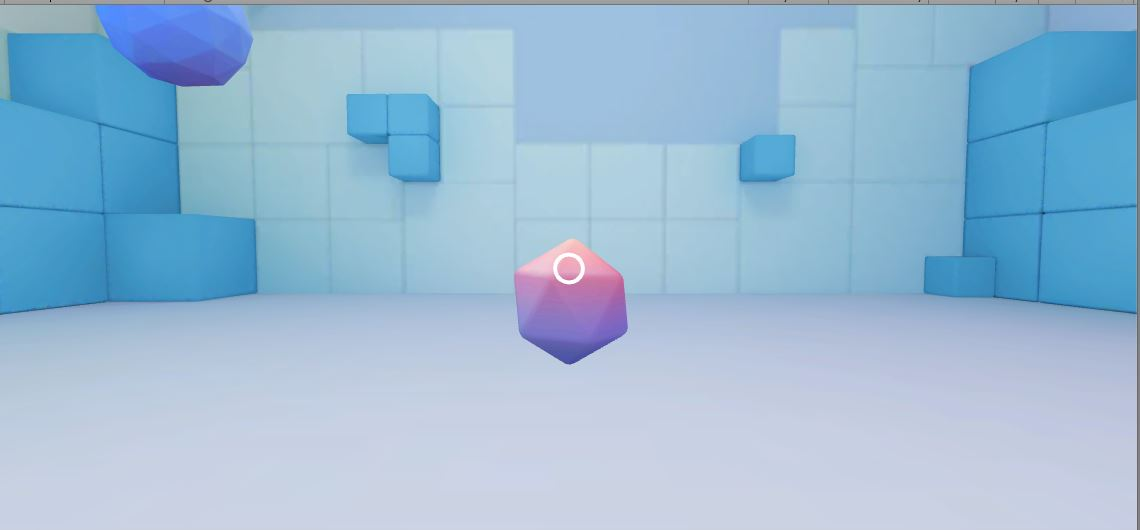
\includegraphics[scale=0.4]{Escena1.jpg}
	\caption{Escena para los ejemplos.}
	\label{fig:Escena1}
\end{figure}

\begin{spacing}{1}
\begin{lstlisting}[float=htbp, caption=Translación y rotación del jugador en el movimiento automático, label=lst:autowalk]
if (isWalking)
        {
            Vector3 direction = new Vector3(mainCamera.transform.forward.x, 0, mainCamera.transform.forward.z).normalized * speed * Time.deltaTime;
            Quaternion rotation = Quaternion.Euler(new Vector3(0, -transform.rotation.eulerAngles.y, 0));
            transform.Translate(rotation * direction);
        }
\end{lstlisting}
\end{spacing}


El segundo \textit{script} \ref{lst:applyForce} consiste en una función que se ejecutará cuando el jugador interactúe con la figura 3D que se puede ver en la figura \ref{fig:Escena1}. Para ello, encontramos el componente \textit{RigidBody}, que es el que nos dejará aplicar una fuerza en los 3 ejes, iterando sobre todos los componentes del objeto. También buscamos la referencia al jugador mediante la función discutida anteriormente \textit{GameObject.FindGameObjectWithTag("Player")}, usando como tag "Player". Obtenemos el componente \textit{RigidBody} del jugador para poder calcular el vector entre los dos objetos, y aplicamos una fuerza en esa dirección, aunque en el eje Y (el que apunta hacia "arriba") se cambia para que la fuerza sea siempre en sentido ascendente. Este ejemplo muestra muy bien cómo se pueden obtener componentes y otros objetos mediante el uso de un par de funciones.

\begin{spacing}{1}
\begin{lstlisting}[float=htbp, caption=Aplicación de una fuerza a un objeto con físicas, label=lst:applyForce]
// Iterate over all components to get RigidBody
Component[] components = GetComponentsInChildren<Component>();
foreach (Component component in components)
{
	if(component is Rigidbody)
	{
		Rigidbody rb = (Rigidbody)component;

		// Calculate vector between player and object
		GameObject player = GameObject.FindGameObjectWithTag("Player");

		Component[] player_components = player.GetComponentsInChildren<Component>();

		Rigidbody player_rb = null;

		foreach (Component player_component in player_components)
		{
			if (player_component is Rigidbody)
			{
				player_rb = (Rigidbody)player_component;
			}
		}

		Vector3 dir =  rb.position - player_rb.position;\\
		Vector3 unit = dir / dir.magnitude;
		unit.y = 0.5f;
		Vector3 force = unit * 250;
		rb.AddForceAtPosition(force, rb.position);
	}
}
\end{lstlisting}
\end{spacing}

El último \textit{script} consiste en la reproducción y pausa de un vídeo interactuando con otro objeto dentro de la escena. En la figura \ref{fig:Escena2} se pueden ver el objeto con el que hay que interactuar y el plano donde se puede visualizar el vídeo. Este último tiene un componente \textit{VideoPlayer} que es el que se encarga de reproducir el vídeo como si fuera una textura dinámica del plano. En el listado \ref{lst:PlayVideo} se puede ver cómo el proceso es prácticamente el mismo: Encontramos el objeto dentro de la escena y obtenemos el componente deseado. En este ejemplo aparece cómo encontrar un componente en concreto sin necesidad de usar un iterador, símplemente estableciendo el tipo específico de componente en la función \textit{GetComponentInChildren()}. Sin embargo, esto sólo funcionará con los componentes de tipos ya definidos en \textit{Unity} (no con otros \textit{scripts}). 

\begin{figure}[htb]
	\centering
	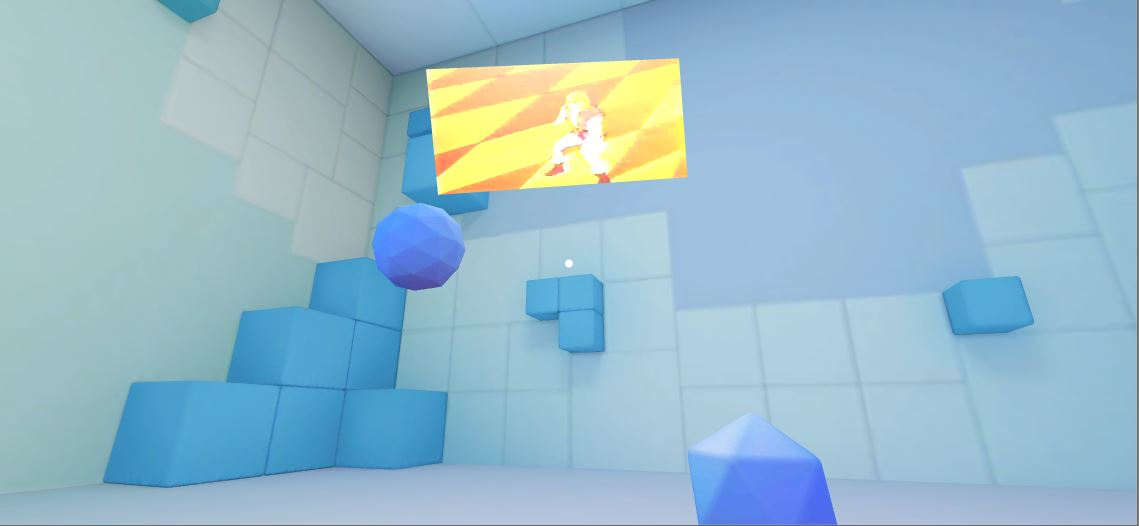
\includegraphics[scale=0.4]{Escena2.jpg}
	\caption{Escena para los ejemplos, segunda perspectiva.}
	\label{fig:Escena2}
\end{figure}

\begin{spacing}{1}
\begin{lstlisting}[float=htbp, caption=Inicio y pausa del vídeo desde el objeto con el que se interactúa, label=lst:PlayVideo]
GameObject video = GameObject.FindGameObjectWithTag("Video");

var videoplayer = video.GetComponentInChildren<UnityEngine.Video.VideoPlayer>();

if (!videoplaying)
{
	videoplayer.Play();
	videoplaying = true;
}
else
{
	videoplayer.Pause();
	videoplaying = false;
}
\end{lstlisting}
\end{spacing}

\section{Conclusión}

La conclusión de este estudio es que Unity es muy flexible tanto en la interacción como en la inclusión de elementos multimedia. 

Algunas de las facilidades que Unity provee para la interacción es la inclusión por defecto de los eventos más usados en el desarrollo de juegos.

Respecto a las facilidades con los elementos multimedia destaca el amplio soporte a formatos tanto de audio como de video y la manera unificada de controlar estos aspectos, sin que sea necesario tener en cuenta el formato del elemento.

\clearpage

%\phantomsection  % OJO: Ojo necesario con hyperref.
\addcontentsline{toc}{chapter}{\refname} % Añade la bibliografía al Índice de contenidos.
%---
% Opción 1: Bibliografía con todas las fuentes en un apartado.
%---

\nocite{*}
\printbibliography

\end{document}

% Local Variables:
% coding: utf-8
% mode: flyspell
% ispell-local-dictionary: "castellano8"
% mode: latex
% End:
